\chapter{DRSSTC}
\label{DRSSTC}

\begin{figure}
    \centering
    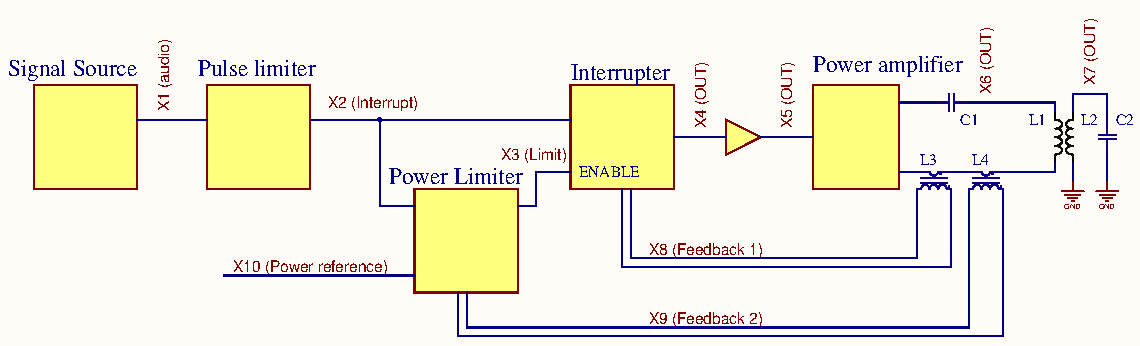
\includegraphics[width=\textwidth]{Skjema/FunksjonsBlokkskjema.pdf}
    \caption{Block diagram}
    \label{fig:func_block}
\end{figure}

\begin{figure}
    \centering
    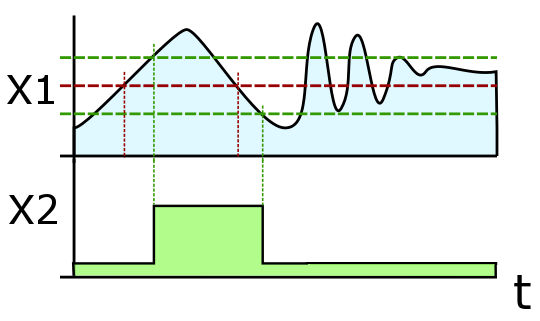
\includegraphics[width=\textwidth]{img/Smitt_hysteresis_graph_x1_x2.png}
    \caption{Tranformation of $X1$ to two level \citep{wikimedia}}       
    \label{fig:schmidt}
\end{figure}


DRSSTC is an acronym for Dual Resonant Solid State Tesla Coil. Dual resonant means that we have two resonant circuits inductively coupled, and tuned to the same resonance frequency. Solid state means that we drive these resonant circuits actively with transistors. The origins of the DRSSTC is not well documented but it is commonly accepted that it was conceived on "The tesla coil mailing list" \citep{pupman}.

The signal pathway consists of a signal source, pulse limiter, power limiter, interrupter, amplifier, and power amplifier see \cref{fig:func_block}.
The signal source provides the signal to be output on the coil, often the signal source is a musical recording.
The input signal should be monophonic, arpeggio\footnote{The sounding of the notes of a chord in rapid succession instead of simultaneously.} may be used. The input signal may be two level.

First the input signal $X1$ goes into the pulse shaper, which transforms the signal to two, level limits on-time of each pulse, and enforces a minimum time between pulses. In \cref{fig:schmidt} an example $X1$ is shown and a corresponding $X2$, here we see that the transformation to two level is done with a schmitd trigger, and that the pulses following immediately after the first pulse is suppressed. Then the signal $X2$ is connected to the interrupter which on a positive flank on $X2$ drives the resonant circuit at its resonant frequency until either the input pulse $X2$ goes low or the limit signal from the limiter $X3$ goes low.
The limiter measures the current flowing through $C_1$ and $L_1$. If the current exceeds a preset level $X10$ the limit signal $X3$ is set low until the next rising edge of the input signal $X2$. $X10$ is set by a multi turn potentiometer.

The resonant circuitry consists of $C_1$, $L_1$, $C_2$ and $L_2$, where $L_2$ is magnetically coupled with $L_1$ with a coupling coefficent of approximately $k=0.2$. $C_1$ is a bank of capacitors with high voltage and current rating and low equivalent series resistance (ESR). $L_1$ is an inductor with high cross section area and few turns (in the magnitude of 5 turns). $L_2$ is an inductor with low cross section area and a high number of turns (in the magnitude of 4000 turns). $C_2$ consists of a sphere or toroid for one plate, and the grounded (safety ground) surroundings. Ground is connected through the safety ground in the electrical socket used to power the DRSSTC. $L_3$ and $L_4$ are current sensing transformers used for feedback.

%Figure \cref{fig:scope} shows a measurement of these signals. Channel 2 (Green) shows the feedback signal $X8$ after it is fed through a protection network limiting the voltage (See the schematic for TK514 in appendix B). Channel 4 (Red) shows an internal signal $Y1 = X2$ \&\& $\overline{X3}$ in the interrupter. As long as this signal is high the output signal $X4$ will swing at the resonant frequency. Note that we would expect $X8$ to be zero as long as channel 4 is low, but there is some delay before the resonant circuit stops swinging after the supply of energy stops. Also note the interference on $X3$ and $Y1$ from the output signal $X6$.

%\begin{figure}
%    \centering
%    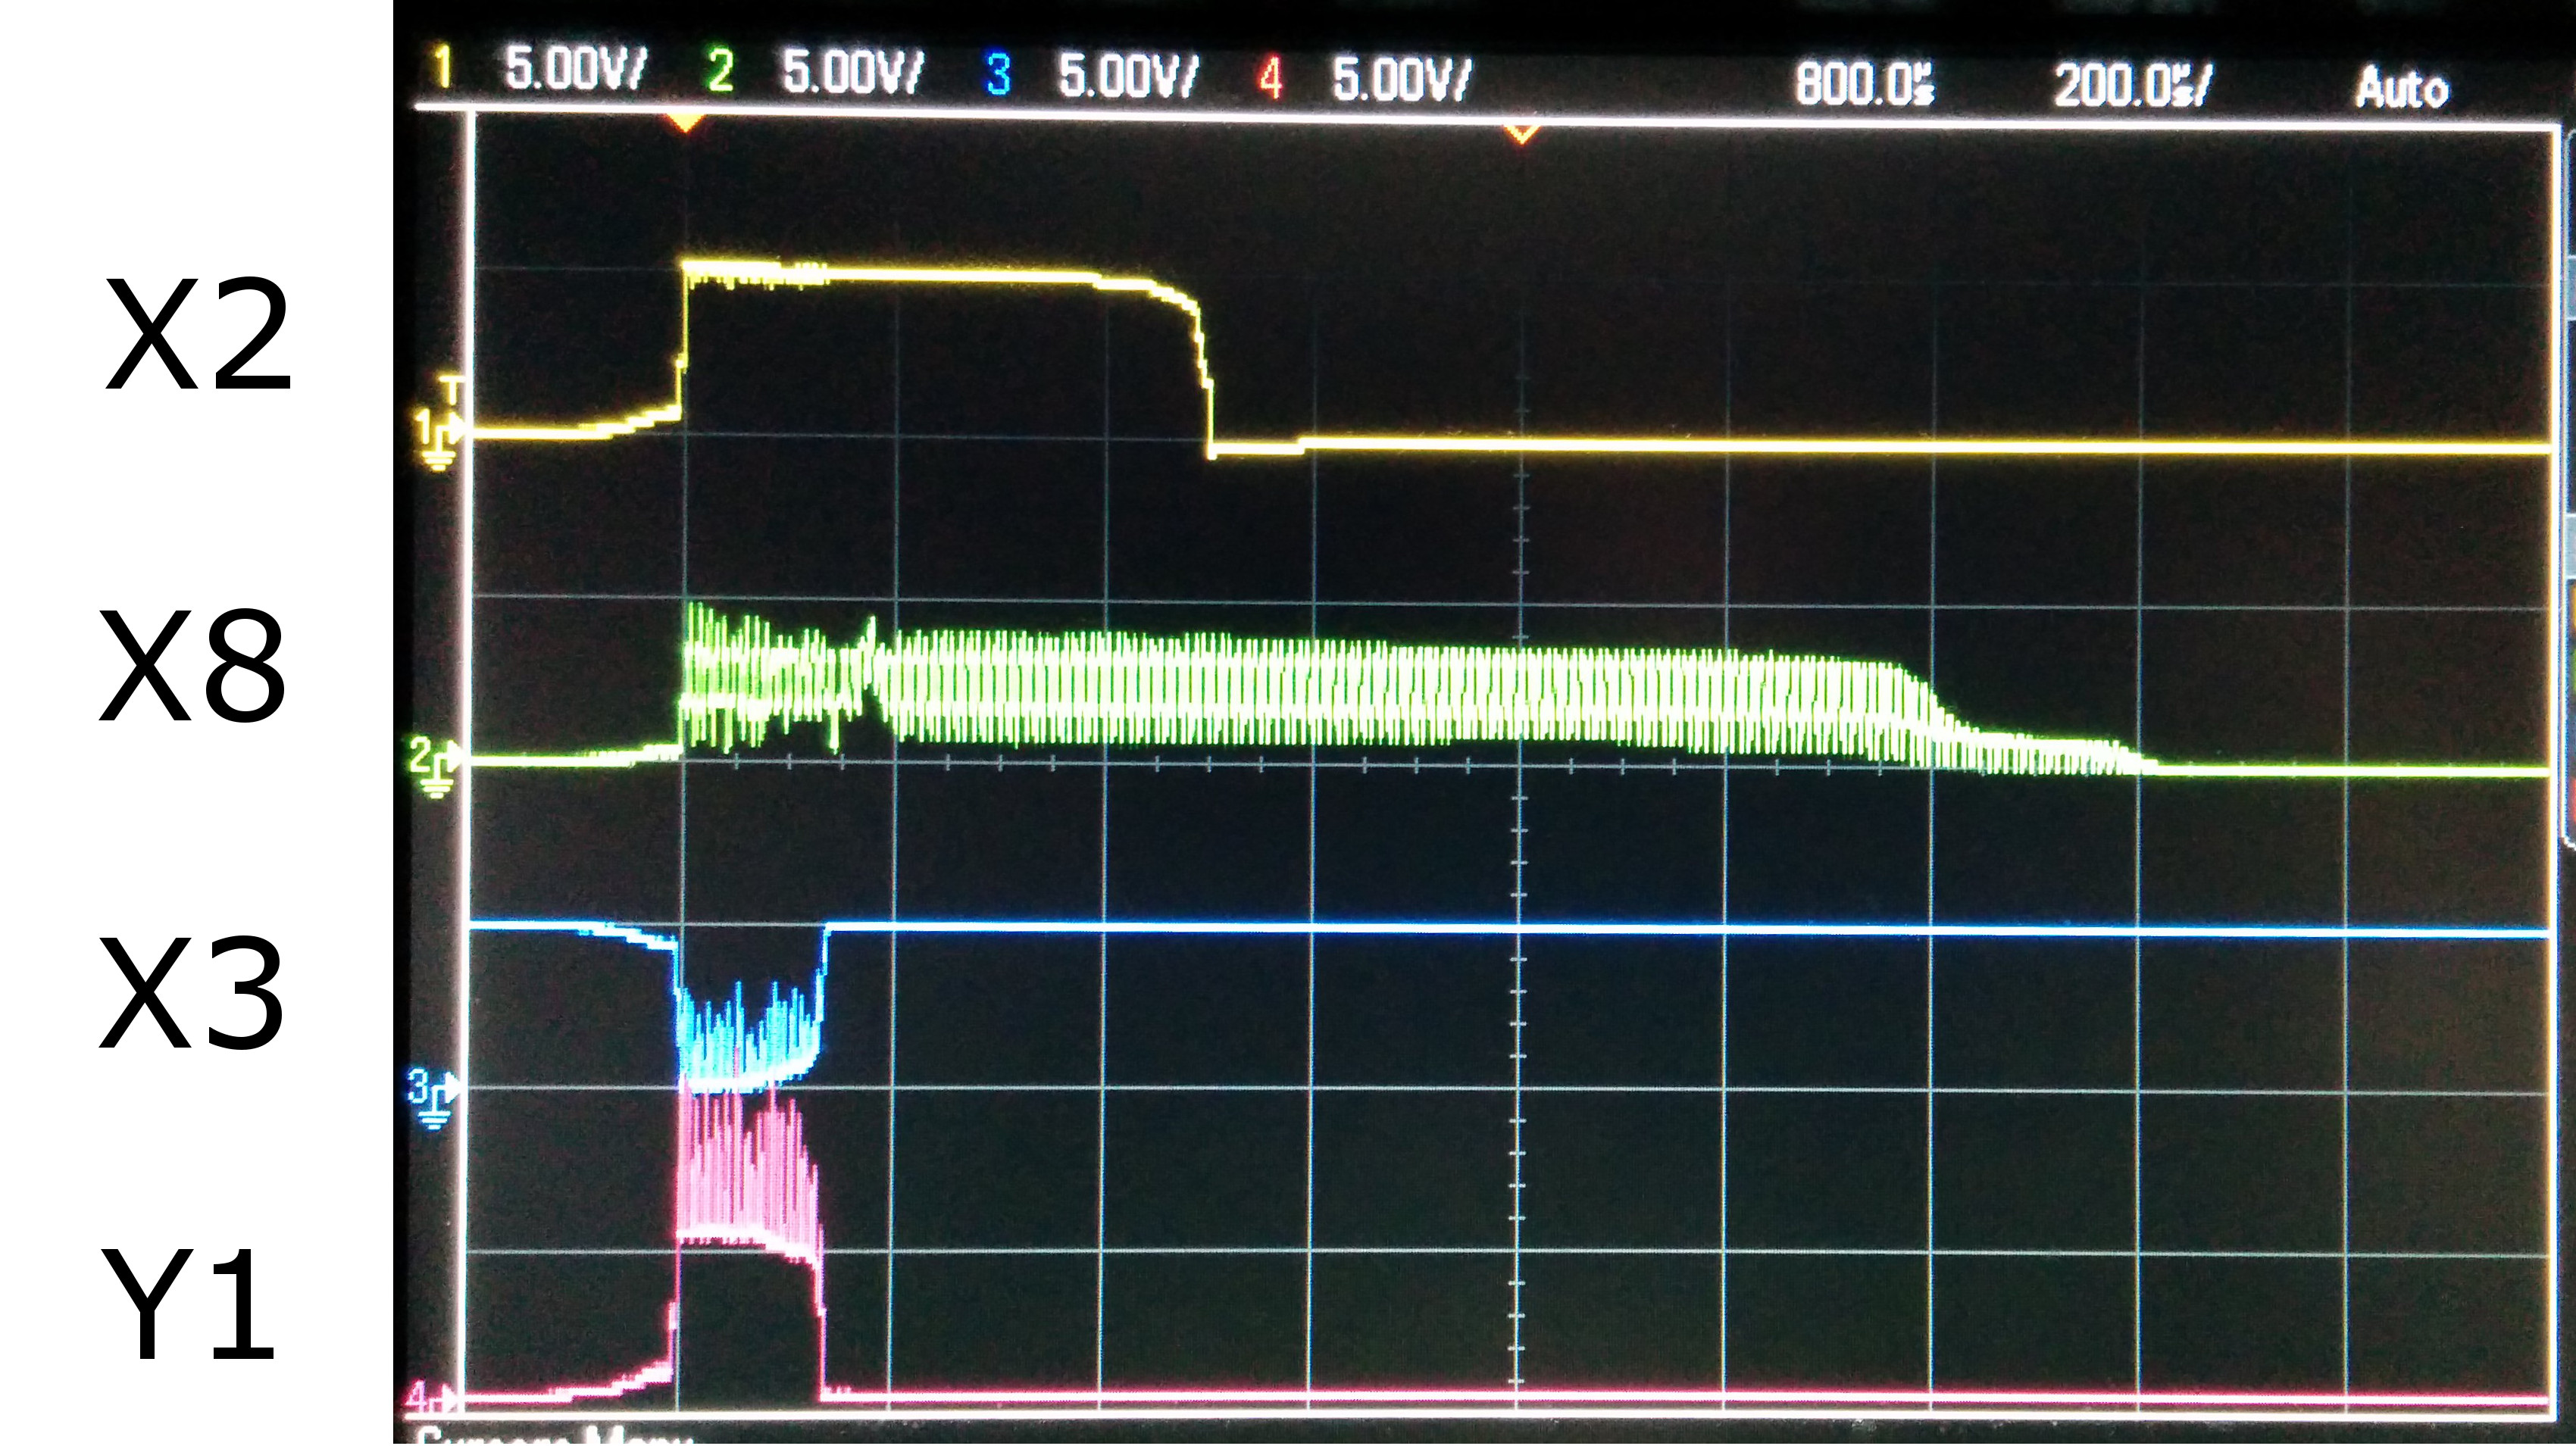
\includegraphics[width=\textwidth]{img/DRSSTC_scope.jpg}
%    \caption{Measurements of signals.}
%    \label{fig:scope}
%    Channel 1 (Yellow): $X2$, 2 (Green): $X8$, 3 (Blue) $X3$, 4 (Red): $X2$ \&\& $\overline{X3}$. Voltage axis: 5V/div. Time axis: $200\mu$s/div.
%\end{figure}
